\chapter{Aggregating Content: A Lightweight Model for Scalable Clustering of Events}

The sheer amount of newsworthy information published by users in social media
platforms makes it necessary to have efficient and effective methods to filter
and organize content. 
%
In this scenario, off-the-shelf methods fail to process large amounts of data,
which is usually approached by adding more computational resources. 
%
Simple data aggregations can help to cope with space and time constraints,
while at the same time improve the effectiveness of certain applications, such
as topic detection or summarization. 
%
We propose a lightweight representation of newsworthy social media data. 
%
The proposed representation leverages microblog features, such as redundancy
and re-sharing capabilities, by using surrogate texts from shared URLs and
word embeddings.
%
Our representation allows us to achieve comparable clustering results to those obtained by using the complete data, while reducing running time and required memory.
%
This is useful when dealing with noisy and raw user-generated social media data.


\section{Introduction}
\label{sec:introduction}

%\mq{hablar de multimodal summarization, diferentes tamaños de topicos, clustering incremental, 
%redundancia ayuda a word embeddings?, complejidad de otros metodos}

%%%%% Index
% Context
% Motivation
% Problem statement
% Contributions

%%%% Content


% Context 
% \subsection{context}

%Un modelo de "representacion" de informacion (de evento en SM) de manera compacta 
%para incorporar nuevo conocimiento.... con aplicaciones A, B y C

%Una forma de modelar la informacion .... (alto nivel)
%Describir semi-formalmente el modelo 
%Poder separar "señales" o "aspectos" del evento 

%Presentar casos de estudio que muestren las N aplicaciones. Mostrar ejemplos de 
%cada aplicacion.

%ej, aplicacion "event retrieval": dado un evento, identificar contenido relevante, topicos o aspectos
%relevantes al evento real (?) 

%modelo con WE exacerba diferencias en los documentos para separar topicos usando UCG (redundancia)

%hipotesis con respecto a agrupar por url: contenido relevante es mas probable de ser compartido con las mismas
%urls que contenido no relevante 


% Nowadays, social media platforms have become a main source of news. According to
% a recent survey, by 2018 about two thirds of US adults used social media as a
% source of news~\cite{pewresearch}, and about 70 percent of Twitter users get
% news from there. With their scale, popularity, and ease of use, social media
% platforms have drastically lowered the entry barriers to disseminate newsworthy
% information in real time. 
%Due to that, news events are often reported earlier in
%social media than in traditional news media. 

% In particular, impactful or breaking real world events (such as the 2015 Nepal
% Earthquake or the 2017 Brexit) overflow social media with millions of messages.
% For that reason, it is a hard task for humans to go through every message in
% order to understand what an event is about. 


The sheer amount of newsworthy information published by users in social media
platforms makes it necessary to have efficient and effective methods to filter
and organize content. 
%
In this scenario, off-the-shelf methods fail to process large amounts of data,
which is usually approached by adding more computational resources. 
%
Simple data aggregations can help to cope with space and time constraints,
while at the same time improve the effectiveness of certain applications, such
as topic detection or summarization. 


%
We propose a lightweight representation of newsworthy social media data. 
%
The proposed representation leverages microblog features, such as redundancy
and re-sharing capabilities, by using surrogate texts from shared URLs and word embeddings.
%
Our representation allows us to achieve comparable clustering results to 
those obtained by using the complete data, while reducing running time and 
required memory.
%
This is useful when dealing with noisy and raw user-generated social media data.


The overload of information in social media streams makes it difficult for users
to obtain a comprehensive account of different emerging events reported by
users.
%
%to get a complete picture of an event or find relevant messages.
%
The ability to identify and summarize relevant information about newsworthy
topics that are accounted for by users in social media can be of great use to
society.
%
This is particularly true in the case of high impact and breaking news, like
natural disasters and crisis situations~\cite{ICWSM1817816}.
%\bp{agregar mas citas}.
%
In general, social media platforms present their content to the consumer in one
of two ways: (1) by displaying user posts in reverse chronological order, or (2)
by displaying posts in a personalized fashion, showing first what they deem more
interesting to the user.
%
However, if the user 
%consuming social media content 
is seeking information about a specific event, the aforementioned approaches can
result also in unnecessary exposure to redundant, irrelevant, or even misleading
information.
%
In this context, delivery of key pieces of information to the user is important,
and even critical in some cases; 
%
for instance, social media is often used as a complementary source of
information for disaster management and
response~\cite{ICWSM1817816,Sarmiento:2018:DDE:3201064.3201077}
%\bp{agregar citas}
and also to obtain information about newsworthy events not yet reported by
formal news outlets. 
%
%In this sense, thThis need to produce high-quality real-time information requires effective ways to filter and organize information about real-world events on social media.
%

Despite the usefulness of social media as a worldwide news information source,
its consumption is not without challenges.
%
These challenges include, among many others, correctly assessing information
veracity and relevance to a specific topic, as well as dealing with a huge
volume of data with variable quality. 
%
%In this sense, the consumption of social media content for information seeking about particular events requires effective ways to filter and organize streaming data.
%%
%
%Specifically, the task of organizing and filtering
%
%Filtering and organizing information in social media can be a
%particularly challenging task.
%
In particular, we study Twitter, in which users can post text-based messages.
%
These messages, called {\em tweets} can include links to images, videos, to
external web-pages or to other tweets, making this platform's content multimodal.

%
%From the perspective of understanding current events, tweets contain a large volume of irrelevant and redundant content, which can often be misspelled, or unreliably capitalized, 
%
%On the other hand, we observe several 
The URLs shared in Twitter often link to varied types of media (articles,
images, or videos), which have been found useful for identifying conversation
topics~\cite{mishne2012twanchor}.
%
In the context of news events, users tend to quickly re-share information if the
event sparks high interest (see Section~\ref{subsec:info_forwarding}), which
results in many (near-)duplicate messages.
%
Dealing with content of these characteristics requires different approaches
than with traditional media~\cite{Alonso:2017:WHH:3091478.3091484}.
%
Prior work has acknowledged the need of techniques for dealing with this type of
social media data.



%%


In this work we focus on the problem of producing summarized representations of
social media data related to news events without significant loss of
information.
%
We present a compact representation for social media content related to news
events.
%
This representation allows us to preserve information about the topics involved
in an event, and to identify relevant content, while reducing the volume of
data.
%
This can be especially useful for online data processing about developing news
and news information seeking tasks.
%
To achieve this, our model annotates shared URLs with the text of the messages
in which they appear.
%
Here we use messages as {\em anchor text} or {\em surrogate text}. 
%
We first leverage this idea by identifying relevant URLs that are shared in
social media during a news event.
%
We discard URLs that are too general with respect to an event (e.g. a general
report), or generic (e.g. linking to the homepage of a news outlet) as we deemed
them as non-relevant.
%
Then we aggregate all the anchor texts associated with relevant URLs into {\em
documents}, and all the conversations around those documents as well. 

As a preliminary way to study the usefulness of our event representation, we
applied it to three news events as a case study.
%
We observed that our representation reduces the amount of records needed to
describe an event by one order of magnitude, compared to using the raw tweets. 
%
We were also able to identify sub-topics by clustering the documents using dense
word representations, such as neural network--based word embeddings. 
%
We show that the clustering based sub-topic detection task using our proposed
representation yields similar external quality metrics to those obtained using
the entire data. 
%
Hence, indicating that we are preserving relevant aspects of the information
while considerably reducing running time.

\paragraph{Contributions.} Our contributions in this chapter are the following:

\begin{enumerate}
  \item We present a novel compact representation for news event information in
  microblogs, based on shared URLs. This representation reduces data volume.

  \item We study the usefulness of our representation through three case
  studies. We do so by introducing a methodology to represent news events in
  Twitter and find sub-topics. We show that our approach displays comparable
  performance to baseline methods at a fraction of the computational resources.
\end{enumerate}


% problemas con representar social media content
% Representing content generally involves representing its constituent terms in
% another space. For instance, using weighted term frequency vectors, graph
% models, or probabilistic models over the distribution of terms. In social media,
% these methods result in highly dimensional sparse features, which are difficult
% to manage without large quantities of well-curated messages. On the other hand,
% it is not trivial to manage large scale data. Current methods can manage large
% volumes of messages at great computational expense or by splitting the dataset
% in smaller sets and dealing with them separately. For example, traditional ways
% of representation of text, such as term frequency weighting, involves the
% generation of thousands of dimensions on messages that are about 10 to 20 words
% long.

% Nonetheless, in the context of news events, user-generated content can be leveraged
% to estimate the relevance of the information and to annotate content from
% external sources. We start from the assumption that users share and comment on
% content that is relevant or interesting to them. Hence, the existence of several
% messages on a topic suggests that the topic is important to users. We can
% leverage this idea even futher: we can annotate the shared URLs in user posts
% with the same text that users put in the posts that contains those URLs. In the
% literature, the text that accompanies a URL is usually known as {\em anchor text}, or
%   {\em surrogate text}, and this idea has been extensively used in query log
% mining~\cite{Beeferman:2000:ACS:347090.347176,10.1007/978-3-540-30192-9_58}. We
% can also take advantage of the redundancy of posts in social media. When exposed
% to an emergent news, users tend to share information as quickly as
% possible~\cite{kalyanam2016prediction}, and this often results in duplicate and
% near-duplicate data. This information can be useful to assess the
% importance of certain aspects of the event. In this work, we exploit these clues
% in order to design a model to represent newsworthy information.

% reescribir
% We propose a lightweight representation of news events in Twitter by aggregating
% tweets based on the existence of shared URLs. Our representation groups tweets
% by common shared URLs into {\it components}, and also ignoring highly common
% URLs in the dataset, in order to avoid having large components of unrelated
% tweets. This representation reduces the amount of records to be processed by one
% order of magnitude, and we validate its capabilities by performing clustering on
% three selected news events to identify sub-topics. By using dense
% representations of words, such as neural network based word embeddings, our
% model generates a compact representation of news events. We show that we achieve
% similar performance on sub-topic detection at a fraction of the time and memory
% required. Our proposed representation allows us to process raw, un-curated
% Twitter data faster than with using individual tweets, and it is flexible enough
% to incorporate new data as the event evolves in time.

% We propose a simple model to represent information about news events in Twitter
% using aggregations of tweets that mention the same URLs, and that retweet or
% reply themselves. Then, we model the resulting sets of documents using dense
% vector representation of terms, such as neural word embeddings, using a corpus
% of 193 million news-related tweets. With this representation, we exploit
% features often discarded in similar works, such as repeated messages and URLs
% mentioned in tweets. This results in a smaller and more flexible representation,
% which allows us to perform some tasks more efficiently, and to incorporate new
% information to the model with little effort. Our event representation is
% compatible with current approaches regarding Twitter event data, such as event
% detection, filtering, and summarization. We show the effectiveness of this
% representation by characterizing topics in news events shared in Twitter, which
% can contain several repeated or irrelevant posts. The topics consist of diverse
% tweets that share URLs, which can be seen as a multimedia representation of
% topics, regardless of the content of these URLs (images, videos, news articles,
% etc.). 




% problemas: mucha info, redundante, etc. 
% explotamos eso para mejorar la origanizacion de la info
% mostramos que es util para: ...
% tiene estas caracteristicas: ...


% One particular problem is what is called information overload: when users are
% exposed to way more information than they can process and understand, and
% effective methods to find relevant information are missing, assuming that
% users know what they are looking for. In this context, automatic summarization
% was proposed as a way to tackle this problem. Given a document or a set of
% documents about a specific topic, the output of the summarization method is a
% gist that summarizes the content, under certain criteria and restrictions. 


% In this work, we approach the issue of information overload by modeling
% content associated with online news, as propagated on Twitter. 
% When a {\em breaking news} occur, users tend to share and
% forward information about it as quickly as possible {\bf REF PLOS}, and ...

% motivation
% \subsection{motivation} 
% user contributed content reflect opinions of users, not media
% importance given by users
% free annotations of urls 




% problems with social media
% \subsection{challenges}
% events are noisy (different levels of relevance)


% However, the scale and rate of publication makes it difficult to understand
% what is happening or what an event is about. Also, the presence of irrelevant
% posts makes it even more difficult to understand a specific event. Usually,
% when a user wants to know about a certain ocurrence, he or she performs a
% search using some keywords, and a chronologically ordered timeline of the most
% recent posts is then shown. In other cases, a special sorting is made in order
% to show the most relevant posts that specific user might like the most, or
% just the posts with the highest scores in terms of popularity. However, this
% is not enough to understand the different aspects or topics related to an
% event.

% Different approaches have been proposed to help users understand the content.
% For example, automatic text summarization is used in order to select the most
% salient phrases from a set of documents, aiming for optimizing diverse criteria,
% such as relevance, coverage, or popularity. However, nowadays online news media
% has increasingly shifted their focus towards multimedia content {insertar
% cita}. There have been some efforts in order to summarize content of different
% modalities, such as images or videos in isolation, but few consider a mixture of
% them. Our hypothesis is that a summary in different content modalities, such as
% images, videos, and text, is more effective than a text-only, or images-only
% summary in order to understand an event. In other words, our hypothesis is that
% a multimodal summary is more informative than a unimodal one. In this work, we
% discuss the challenges of the current approaches and tackle the problem of
% multimedia summarization of events in social media, by considering content
% independently of its nature.



% problem statement
% \subsection{problem statement}

% hypotheses
% \subsection{hypotheses}
% Hypotheses: 
% 1. grouping tweets by url improve the ...
% 2. the use of word embeddings (fasttext) improve the ...

% % contributions
% % \subsection{contributions}
% Our contributions are the following:
% \begin{enumerate}
%   \item We investigate 
%   \item
%   \item ?
% \end{enumerate}


% % outline of paper
% % \subsection{outline}
% This paper is organized as follows. Section ...

% % -----------------------------------------------------------------------

% % Twitter desc
% On Twitter, each post, called {\em tweet}, is a short text ---traditionally
% 140 characters long, but by the year of 2017 this limit was extended to 280
% characters---, which can contain arbitrary URLs, as well as {\em hashtags}
% (words prepended with a \#, serving to the tweet as tags), {\em cashtags}
% (prepended by a \$, serving as identifiers for stocks and shares), and mentions
% (names of Twitter users).

\section{Related Work}\label{sec:related}
% There is extensive work on automatic summarization on microblogs\mq{ref}. In
% this work, we approach the problem from a practical point of view, where our
% goal is to benefit from the characteristics of social media posts, in
% particular, from event-related messages. We exploit the redundancy of
% information available in social media via the aggregation of information
% around shared URLs, and propose a simple and compact model using word
% embeddings on tweets. Therefore, we can classify the related work in three
% areas: modeling social media content, automatic summarization of news, and
% usage of word embeddings in social media.

Two lines of research are relevant to our work: the utility of anchor texts in
microblogs and topic detection methods using different aggregation strategies. 

%\bp{No hay literatura de representaciones compactas de eventos para sumarizacion?}


%%%%% Studies from 201x have shown that around 25\% of tweets contain at least one URL.
There have been studies about the usefulness of anchor texts in Twitter. 
%
Raux et al.~\cite{raux2011describing} used anchor texts from tweets pointing to a
predefined set of URLs to characterize general topics, by clustering a bipartite
graph of words and URLs. 
%
We instead focus on news events, and tweets related to these news, without using
predefined URLs, but instead the actual shared URLs. 
%
Mishne and Lin~\cite{mishne2012twanchor} studied the
contribution of anchor texts compared to the text of the websites behind the
URLs, concluding that anchor text add new terms not seen in the website content,
by looking also at the conversations around the sharing tweets. 
%
Alonso et al.~\cite{Alonso:2015:WCW:2740908.2745397} had similar findings examining
Facebook posts. 
%
In another work by Alonso et al.~\cite{Alonso:2017:WHH:3091478.3091484}, the authors designed a social search
engine using the propagation of shared URLs as cues to measure virality, and anchor texts to augment metadata of the search results with social
content. 
% In a previous work~\cite{quezada2013understanding}, we showed a
% prototype of a multimodal summarization methodology using anchor texts. In this
% work, we do not make use of or compare to the content of the URLs themselves,
% but use solely the anchor texts as a mean to represent the content about a news
% event.

Topic modeling of tweets is an active line of research, and there are some
studies which investigate the effectiveness of aggregation of tweets to improve
topic
detection~\cite{Hong:2010:EST:1964858.1964870,Mehrotra:2013:ILT:2484028.2484166,alvarez2016topic}.
Hong and Davison~\cite{Hong:2010:EST:1964858.1964870} analyzed the effects of
different aggregation strategies of tweets when finding topics with Latent
Dirichlet Allocation. They found that some schemes yield better results at some
tasks, such as classification problems related to tweets. In a similar fashion,
Mehrotra et al.~\cite{Mehrotra:2013:ILT:2484028.2484166} observed that
aggregating hashtags (also denoted as {\em pooling} of tweets by hashtags) is a
more effective strategy to identify topics from tweets, but at the cost of
longer running times due to the duplication of tweets. Finally, Alvarez-Melis
and Saveski~\cite{alvarez2016topic} found that adding the threads of
conversation into the pooling is more effective than pooling by hashtag in their
observations. We instead aggregate by shared URLs and conversations, yielding
similar performance to our baseline, with reduced running time.



% \subsection{Using common information in tweets}

% Similar to our work, in the sense of exploiting common information across
% messages, the work of Kamath et al.~\cite{Kamath:2013:SDO:2488388.2488447}
% focuses in the spatio-temporal dynamics of {\em memes}, as seen as units of
% information spreaded in social media. For this, they model each tweet as a
% tuple of the hashtags involved, time, and location to observe and characterize
% topics in Twitter. Similarly, the work of Pe\~na-Araya et
% al.~\cite{pena2017gaining} aim to characterize geopolitical entities (such as
% countries) based on the tweets that mention them, by proposing a model to
% represent locations in a spatio-temporal ambit, and develop a visual analytics
% tool to explore events based on the location scope of their impact. Our work
% is similar to both in the sense of leveraging common entities across messages,
% in this case, the URLs, in order to generate a compact representation to
% facilitate the discovering of sub-events. In our case, we do so by using URLs
% and the text content as a surrogate for the URLs, also called anchor texts.

% Concerning the specific use of anchor text in social media, Mishne and
% Lin~\cite{mishne2012twanchor} show that the anchor texts in general tweets
% provide additional new information compared to the content of webpages alone
% in a study of 7 million URLs obtained from the Twitter Firehose. The work of
% Raux et al.~\cite{raux2011describing} is one of the first to use anchor texts
% to find clusters of topics in Twitter, in order to describe Web content using
% tweets. The authors create a weighted bipartite graph of tweet words and URLs,
% being the weight the tf-idf score of the words in the tweets that contain the
% URL, and then find clusters of URLs. Although they characterize clusters of
% URLs as topics, their work focuses on general tweets and not newsworthy
% messages in particular. In the work of Alonso et
% al.~\cite{Alonso:2017:WHH:3091478.3091484}, the authors develop a search
% engine for content related to URLs shared on Twitter, displaying the most
% popular and viral URLs, also showing the effectiveness of this approach. In
% our previous work~\cite{quezada2013understanding}, we show a prototype of a
% automatic summarization methodology using tweets aggregated by URL, and then
% modeling the aggregated sets as tf-idf vectors to cluster them, find sub-events, 
% and then selecting the most representative messages as a multi-modal
% summary.

% % \subsection{General text representation methods}

% % % verificar
% % %In a general domain, LDA is very good to find/extract topics, but not in the 
% % %domain of this work. So my magnificent research is pretty very much fabulous.

% % Topic models are a useful way to deal with textual information and to derive a
% % low-dimensional representation of documents. One of the most popular methods
% % is Latent Dirichlet Allocation, or LDA~\cite{blei2003latent}. LDA models a
% % document as a mixture of different topics, which are probability distributions
% % on the vocabulary. TwitterLDA~\cite{zhao2011comparing} is a modification to the 
% % original approach, by changing the assumption that a single document can discuss different topics, which may be unlikely in short messages, such as tweets. Our representation is 
% % compatible with LDA or TwitterLDA, as it provides a way to aggregate topical information which can
% % be used as input for topic models.

% % We also use dense word embeddings such as the continuous representations obtained by using shallow
% % neural networks such as {\tt word2vec}~\cite{DBLP:journals/corr/abs-1301-3781} 
% % or {\tt fastText}~\cite{bojanowski2016enriching}. Dense vector representation of words
% % provide a efficient way to assess the similarity of terms or documents. In contrast,
% % traditional methods, such as tf-idf~\cite{Salton:1983:EBI:182.358466}, involve generating embedding of words of thousands of dimensions, as high as the vocabulary size. Some methods, such as
% % Latent Semantic Analysis~\cite{dumais2004latent}, aims to reduce the dimensionality of the representation by doing matrix factorization. In our case, our model aims to generate a representation of low dimensionality by using neural word embeddings over the aggregation of 
% % related messages, and by doing so, reducing the amount of documents.


% \subsection{Applications of tweet representations}

% Automatic text summarization has been employed in different domains, such as
% news~\mq{cite}, sports~\cite{meladianos2018optimization,chakrabarti2011event},
% music~\cite{raposo2016using}, or movies~\cite{aparicio2016summarization}.

% There are several approaches for automatic summarization of events from social
% media, being many of them inspired in automatic text summarization. In order
% to manage scale, most of the related approaches do not deal with all the data
% at once, but work with similar sub-problems, such as sub-events detected via
% time windows, clustering, or online approaches. 

% The work of Chakrabarti and Punera~\cite{chakrabarti2011event} identifies
% particular time windows in structure-rich events, such as football matches.
% Using Hidden Markov Models, the authors find time windows associated with
% specific sub-events (e.g., a "touchdown") and then summarize each sub-event
% using a centroid-based approach on the tf-idf representation of the tweets.
% Similarly, Alsaedi et al.~\cite{alsaedi2016temporal} fix a time window of one
% hour to define all the tweets in that time window as a cluster, and then use
% two consecutive clusters to take into account the changes between time
% windows. They also propose two additional approaches, namely using a retweet
% voting approach and a temporal centroid method. In all cases, the approaches
% do not use all the dataset at once, but select a limited amount of messages as
% a sub-event. 

% We do not follow this approach, mainly because different sub-events  
% may be mentioned in different stages of the event, and the time-window
% approach can result in low purity clusters when being applied to general
% events.


% One of the first online approaches to event detection and summarization in
% Twitter is the work of Sankaranarayanan et
% al.~\cite{Sankaranarayanan:2009:TNT:1653771.1653781}. The authors describe a
% system that collects tweets and identifies events using an online clustering
% procedure over a tf-idf representation of tweets. \mq{problema con esto}




% \mq{completar (eval)} There is no definitive standard against which one can
% compare the results from an automated summarization system. In general, the
% methods for evaluating summaries can be classified in two kinds: intrinsic or
% extrinsic. The first one evaluate the quality of the summary itself, e.g.,
% compare the summary generated by the system with other summaries generated by
% human experts, whereas the extrinsic evaluate how the summary helps the
% accomplishment of another task, such as classification.




\section{Event Representation}\label{sec:model}

We introduce our model and the methodology for applying it to messages that
describe events in social media.

% We introduce a scalable high-level news event representation from microblog data, leveraging
% social media features such as redundancy. Specifically, we define our
% representation and some possible applications.
% The key idea of our representation is to leverage redundancy, common information
% across messages, to reduce the amount of resulting documents while increasing
% the effectiveness of the corpus.
% %, and to be able to easily identify different aspects of an event. 
% For that, we use the shared URLs as clues to aggregate messages into a single
% {\em document}. Our assumption is that the content of the messages that mention
% the same URLs refer to the same aspect of an event. For example, if an URL
% points to an image of a destroyed building (e.g., in the context of an
% earthquake), then it is highly likely that the text of all the messages
% containing that URL will refer to the building and not to a different topic. We
% say that the text in those messages is a {\em surrogate} of the content in the
% URL. This allows us to annotate multimedia content using social media
% information. At the same time, we can reduce the amount of messages by
% aggregating them into a single document, resulting in a more scalable
% representation. 
% We also incorporate other social interactions, such as forward or reply
% messages. For example, in Twitter they are called {\em retweets} and replies,
% respectively. The assumption is similar, and the action of forwarding or
% replying a message can be seen as sharing the URL of the message being
% forwarded or replied, as well.


% Idea: presentar el modelo con la suposicion de que las URLs que tenemos son las
% buenas, es decir, identifican "bien" un topico del evento, a diferencia de las
% urls que no (las que tienen mucho grado en el grafo de coocurrencia). Luego, en
% la metodologia, mostrar una forma de identificar las urls buenas usando el graof
% de coocurrencia.
% tres tipos de urls: "especificas" (topic-specific), generales e irrelevantes

%\paragraph{\bf{Representation definition}}

Our model is based on the assumption that {\em most of the social media posts
that discuss a specific event and contain a URL, are messages that cover a
particular portion or sub-topic of the event}.
%
For example, in the case of an earthquake, tweets that refer to damages to
buildings may share a URL to an external news report; similarly, a tweet that
discusses the magnitude of the event may link to the official seismological
report.
%
We define an event as a tuple $\mathcal{E} = (M, U)$, where $M$ is the set of
messages that discuss a real-world occurrence, and $U$ is
the set of {\em topic-specific} URLs that are mentioned or shared by messages in
$M$. 
%
We denote the URLs $U$ as {\em topic-specific}, assuming that each URL in $U$
identifies only one of the different topics within the real-world event.
%
Our representation is a graph $\mathcal{G} = (V, E)$, where $V \subseteq M \cup
U$ is the set of nodes, comprised of {\em messages} and {\em URLs}, and there is
an edge $(i, j) \in E$ if at least one of the following conditions hold: (1)
$m=i$ is a message and $u=j$ is a URL and $m$ shares $u$, (2) $m_1=i$ and
$m_2=j$ are messages and $m_1$ re-shares $m_2$, or (3) $m_1=i$ and $m_2=j$ are
messages and $m_1$ replies to $m_2$ (see an example in
Figure~\ref{fig:model-example}).
%
Finally, a {\em document} is a connected component of $\mathcal{G}$.
%
In this case, a document is defined as a collection of messages that discuss
only one aspect of the event.

%%

The assumption of $U$ to be a set of topic-specific URLs may not hold in all
cases, for example, for URLs that address general aspects of an event (e.g., a
summary report of an entire event), or that are generic (e.g., refer to a online
news website's root URL), or irrelevant to the event (e.g., spam, or unrelated
information).
%
We deal with these cases in our methodology for generating event models,
presented below.
% In other cases, a message could share more than one URL, and the two of them can
% be complementary, for example, sharing a news report along with a relevant image
% or video.
%
In that sense, our model and methodology focus on identifying URLs that are
specific to one aspect of an event, and use those URLs to aggregate similar
messages.
%
Our goal is to represent underlying sub-topics of an event by just using shared
URLs. 


%%

%\bp{creo que lo anterior esta incompleto y algo confuso: Falta decir que en realidad una componente conexa es un documento (al final esta es la representacion). Tambien hay que decir que en realidad una componente se entiende como elementos que hablan de lo mismo y por eso se modelan como un unico documento. El resto de identificar urls problematicas esta bien que quede en la metodologia.}

\begin{figure}[t]
  \centering
  \resizebox {0.6\columnwidth} {!} {
    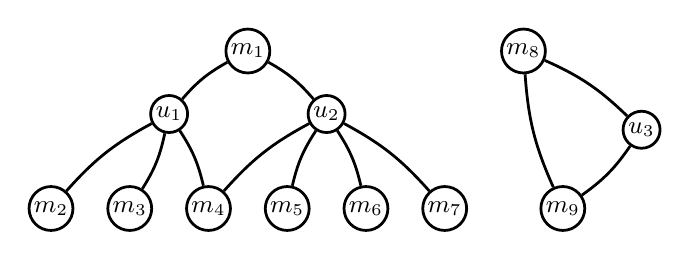
\begin{tikzpicture}[
    every edge/.style={draw, line width=1pt, align=left, sloped}
    ]
  
    \node[draw, circle, inner sep = 1pt, line width=1pt] (m1) at (0, 0) {\small $m_1$};
    \node[draw, circle, inner sep = 1pt, line width=1pt] (u1) at (-1, -0.8) {\small $u_1$};
    \node[draw, circle, inner sep = 1pt, line width=1pt] (u2) at (1, -0.8) {\small $u_2$};
    
    \node[draw, circle, inner sep = 1pt, line width=1pt] (m2) at (-2.5, -2) {\small $m_2$};
    \node[draw, circle, inner sep = 1pt, line width=1pt] (m3) at (-1.5, -2) {\small $m_3$};
    \node[draw, circle, inner sep = 1pt, line width=1pt] (m4) at (-0.5, -2) {\small $m_4$};

    \node[draw, circle, inner sep = 1pt, line width=1pt] (m5) at (0.5, -2) {\small $m_5$};
    \node[draw, circle, inner sep = 1pt, line width=1pt] (m6) at (1.5, -2) {\small $m_6$};
    \node[draw, circle, inner sep = 1pt, line width=1pt] (m7) at (2.5, -2) {\small $m_7$};
  
    \path [-] (m1) edge[bend right=10] node[below=1pt] {} (u1);
    \path [-] (m1) edge[bend left=10] node[below=1pt] {} (u2);

    \path [-] (m2) edge[bend left=10] node[below=1pt] {} (u1);
    \path [-] (m3) edge[bend right=10] node[below=1pt] {} (u1);
    \path [-] (m4) edge[bend right=10] node[below=1pt] {} (u1);
    \path [-] (m4) edge[bend left=10] node[below=1pt] {} (u2);
    
    \path [-] (m5) edge[bend left=10] node[below=1pt] {} (u2);
    \path [-] (m6) edge[bend right=10] node[below=1pt] {} (u2);
    \path [-] (m7) edge[bend right=10] node[below=1pt] {} (u2);


    \node[draw, circle, inner sep = 1pt, line width=1pt] (m8) at (3.5, 0) {\small $m_8$};
    \node[draw, circle, inner sep = 1pt, line width=1pt] (u3) at (5, -1) {\small $u_3$};
    \node[draw, circle, inner sep = 1pt, line width=1pt] (m9) at (4, -2) {\small $m_9$};

    \path [-] (m8) edge[bend right=10] node[below=1pt] {} (m9);
    \path [-] (m9) edge[bend right=10] node[below=1pt] {} (u3);
    \path [-] (m8) edge[bend left=10] node[above=1pt] {} (u3);

  \end{tikzpicture}
  }
  \caption[Example representation of messages.]{
    Example representation of messages. 
    Messages $m_1$ and $m_4$ shares URLs $u_1$ and $u_2$, while $m_2$ only shares $u_1$;
    $m_8$ and $m_9$ share or reply one to another. Each connected component is a {\em document}.
  }
  \label{fig:model-example}

\end{figure}

% \begin{figure}
%   \centering
%     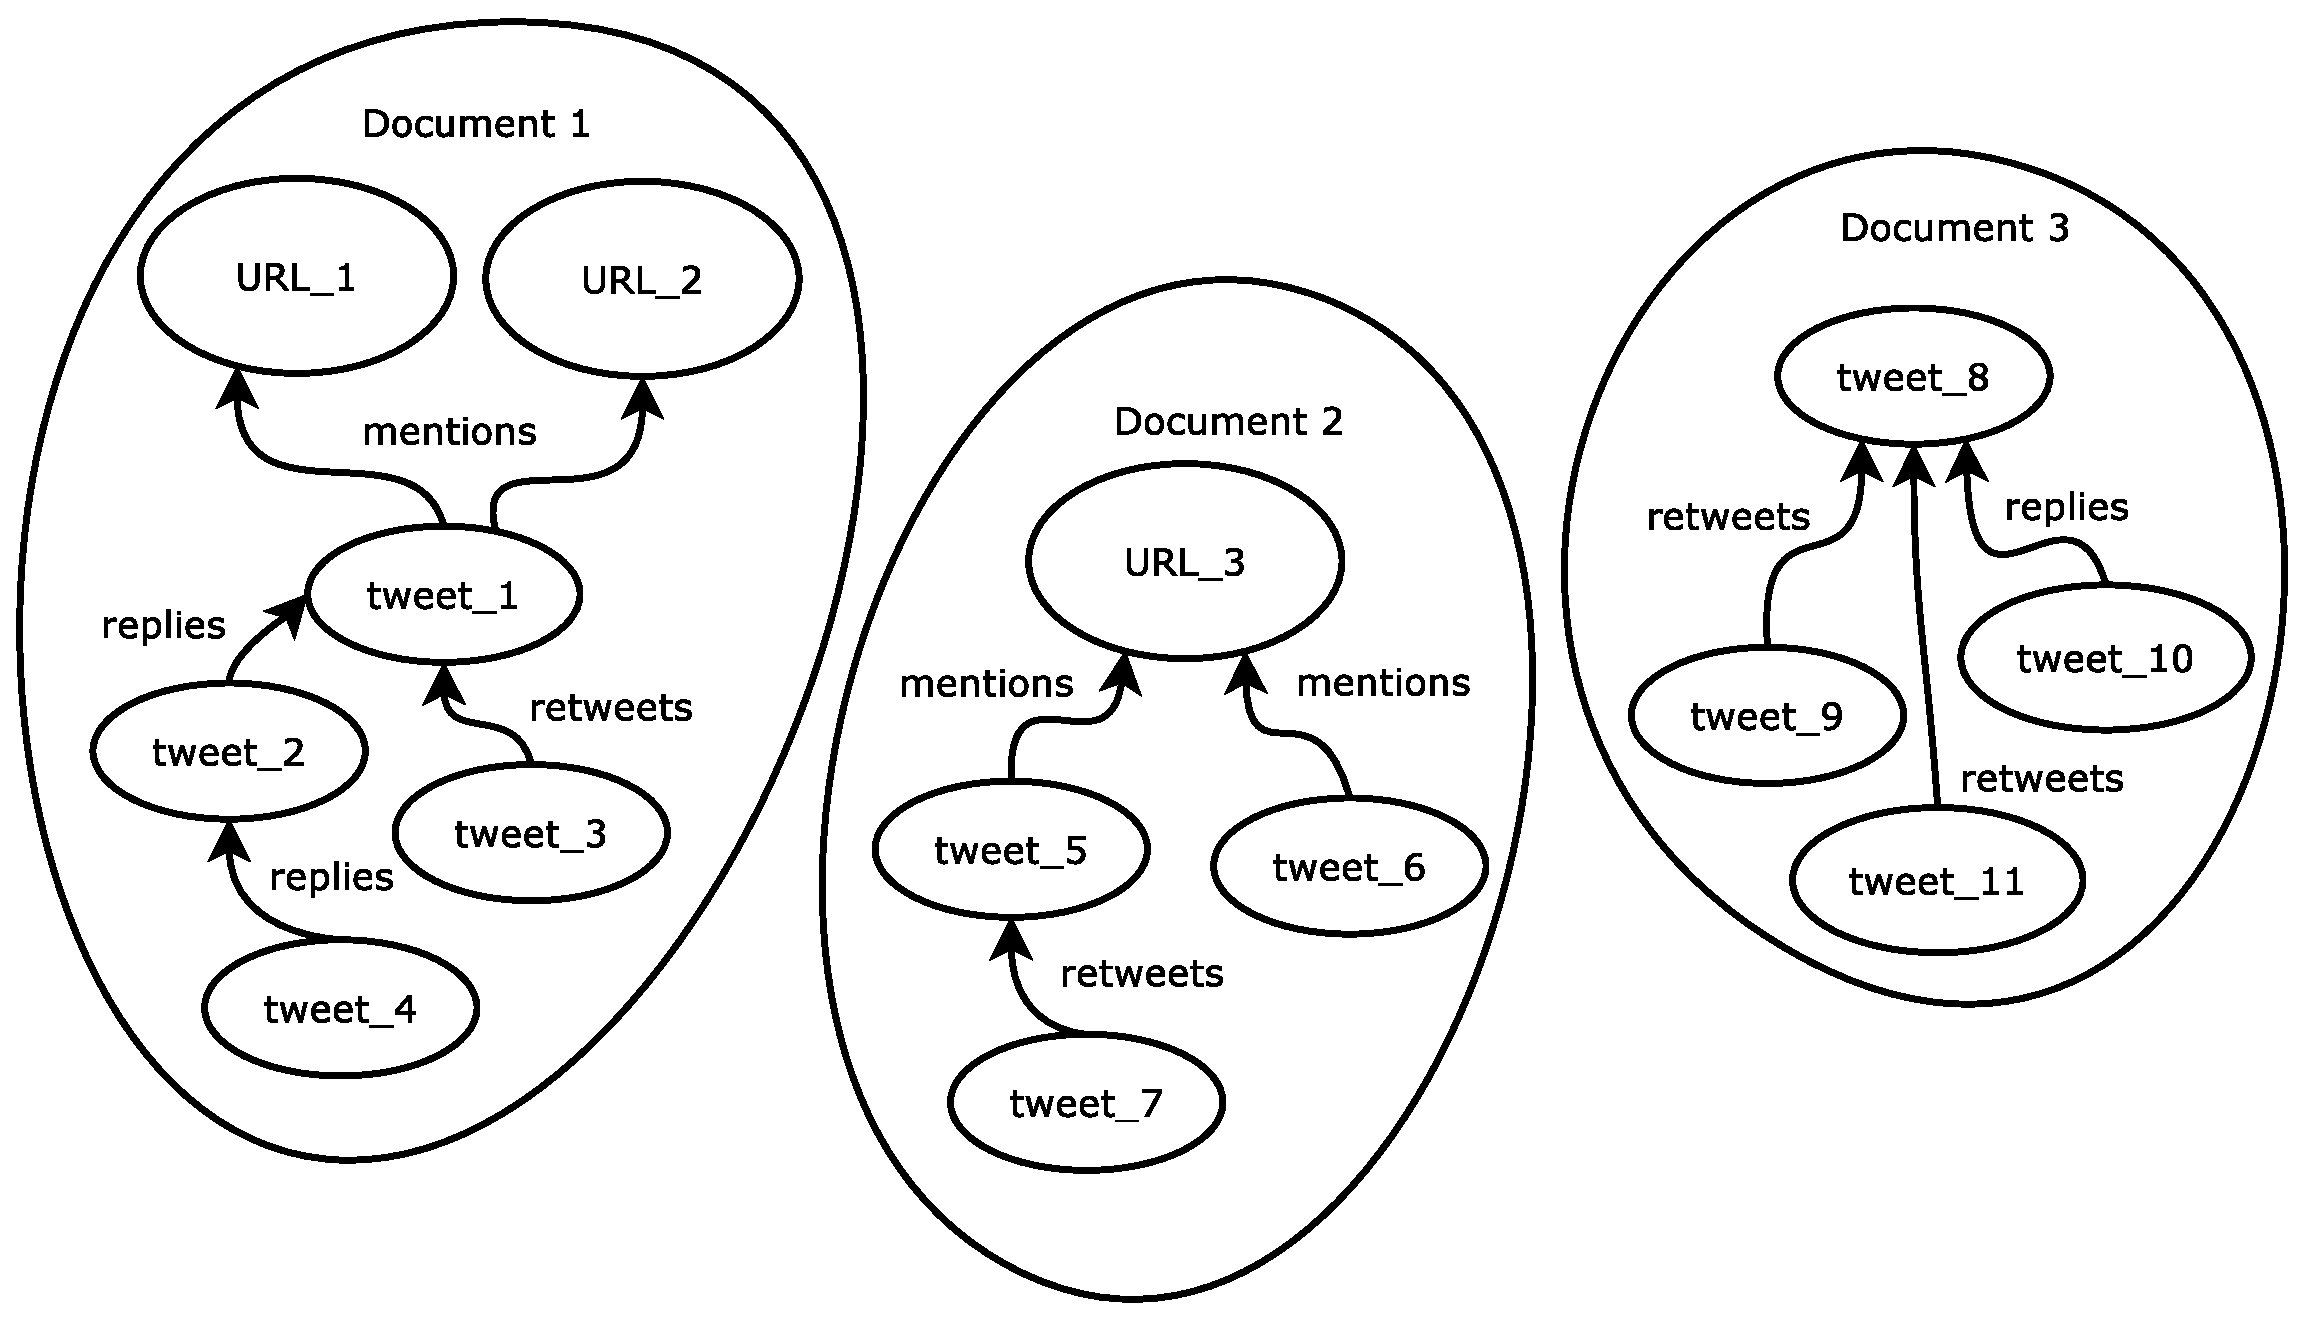
\includegraphics[width=0.4\textwidth]{fig/docs.eps}
%   \caption{Conceptual example of documents. A document is a set of messages that share or reply each other, and the messages that share the same URL. In order to have a representative element for each document, only documents with URL can be considered, and documents with multiple URLs can be duplicated, while each document has a different URL.
%   }\label{fig:model}
% \end{figure}

% Consider Twitter as an example. A document $d$ is a set of URLs, plus the tweets
% that mention those URLs, plus the tweets that retweet or reply any of the
% tweets in $d$. Note that if there are more than one URL, then there should be
% at least one tweet that mention all those URLs, or there is a path of replies
% or retweets between the tweets that mention those URLs individually.
% Figure~\ref{fig:model} shows an example of a few documents.

% \begin{algorithm}
% \caption{Model generation}\label{algo:gen}

% \SetAlgoLined
% \KwData{Messages $T$, URLs $U$ mentioned in messages in $T$}
% \KwResult{Documents $D = \{d_1, d_2, \ldots, d_N\}$, with $d_i\subseteq T\cup U$, for $i\in \{1, \ldots N\}$}
%  $Pairs \leftarrow \emptyset$\;
%  \For{$t \in T$}{
%   \For{$u \in U$ that is mentioned by $t$} {
%     $Pairs \leftarrow Pairs \cup \{(t, u)\}$\;
%   }
%   \If{$\exists t' \in T$ such that $t$ replies to or forwards $t'$}{
%    $Pairs \leftarrow Pairs \cup \{(t, t')\}$\;
%   }
%  }
%  \For{$u \in U$} {
%   \em{UnionFind}.makeSet$(u)$\;
%  }
%  \For{$(p, q) \in Pairs$} {
%   \em{UnionFind}.union$(p, q)$\;
%  }
%  $D \leftarrow UnionFind.sets()$\;
% \end{algorithm}
% \vspace{-0.5cm}

%%%%%%%%%%%%%%%%%%%%%%%%%%%%%%%%%%%%%%%%%%%%%%%%%%%%%%%%%%%%%%%%%%%%%%%%
%%%%%%%%%%%%%%%%%%%%%%%%%%%%%%%%%%%%%%%%%%%%%%%%%%%%%%%%%%%%%%%%%%%%%%%%
%%%%%%%%%%%%%%%%%%%%%%%%%%%%%%%%%%%%%%%%%%%%%%%%%%%%%%%%%%%%%%%%%%%%%%%%
%%%%%%%%%%%%%%%%%%%%%%%%%%%%%%%%%%%%%%%%%%%%%%%%%%%%%%%%%%%%%%%%%%%%%%%%


%\paragraph{\bf{Generation methodology}}\label{sec:methodology}

\subsection*{Methodology for representing events}

Given a set of event-related social media messages, we propose the following
methodology for representation generation:
  
{\bf Filter out generic URLs:} 
%
We identify generic URLs (too general with respect to the event) as those that
co-occur with several different other URLs in the same messages. 
%
%A URL co-occur with another one if they both are shared by the same message.
%
Highly connected URLs do not contribute to specific topics: links that are very
generic (e.g., {\tt cnn.com}) or very general to the event (e.g., general
reports). 
%
All of the messages mentioning these URLs would fall into the same component,
regardless of their differences in content. 
%
We removed URLs that co-occurred with three or more different URLs across
messages.
%
This threshold yielded the best results in our case studies.


{\bf Representation generation:} 
%
The generation step consists of grouping messages that end up in the same
component, as described in the previous section.
%
For that, a straightforward method is to compute all pairs of messages and pairs
of URLs and messages that fulfill the conditions stated in the representation
definition and then find connected components using a union-find algorithm.
%
The URLs are the non-generic ones identified in the previous step, as an
approximation to the topic-specific URLs.


{\bf Vector representation of documents:} 
%
Finally, we aggregate messages into documents in order to produce a vector
representation, using neural network-based word embeddings.
%
This procedure generates dense document representations.




% Our goal is to propose a methodology for generating automatic summaries from
% news events on Twitter, exploiting both the multimedia content and the
% importance that users give to certain topics. For that, we learned a
% representation of the URLs shared from event-related tweets (URLs pointing to
% images, videos, other tweets, or other Web pages in general), using the text in
% the tweets that surround those URLs, borrowing the idea of anchor texts in query
% log mining. We used this representation to group the URLs into clusters and then
% used the social features of each tweet in order to rank the URLs and the
% clusters, based on the level of activity that users had on each of those. This
% allowed us to sort the different aspects of an event based on the importance
% that users give to them.



% \subsection{Definitions}

% \paragraph{Tweet} A {em tweet} can be seen as a struct with the following fields:

% \begin{itemize} \item {\em text}: the textual content of the tweet. \item {\em creation\_date}: a
% timestamp when the tweet was published. \item {\em no\_retweets}: the amount of times that tweet was
% shared or       forwarded by other users. \item {\em no\_likes}: the amount of times users ``liked''
% the tweet. \item {\em user}: an identifier of the user who published the tweet. \end{itemize}


% \paragraph{Summary} Given a set of tweets $E = \{t_1, t_2, \ldots, t_N\}$, called an {\em   event},
% we want to select a subset $S \subseteq E$ of tweets, called   a {\em summary}. The summary must
% fulfill the following criteria:

% \begin{itemize}      
% \item {\bf Topical coverage}: the tweets in $S$ must cover the same topics as
% $E$.   \item {\bf Redundancy}: the content of tweets in $S$ must not be redundant with each other.

% \item {\bf Importance}: the tweets in $S$ must be the top $|S|$, with respect to $E$, according to a
% pre-defined ranking function, considering into account the previous two criteria. For example, if
% two tweets have the same value according to the ranking, but     the two of them are equal in terms
% of content, then only one of them should be in $S$.   

% \item {\bf Human-manageable size}: the size of
% $S$ must be of much less size than $E$, only if $E$ is large. {\bf (TODO: define what is ``large''
% and how less is ``less.'')} \end{itemize}

% \paragraph{Replies and retweets} We denote by $\mathit{URL}(t) = \{u_1, u_2, \ldots, u_m\}$ the URLs
% shared by the tweet $t$. $\mathit{URL}(t)$ is empty if $t$ does not share any URL.

% We also denote by $\mathit{replies}(t)$ the set of all tweets $t'$ such that $t'$ is a {\em reply}
% of $t$, or $t'$ is a reply of another tweet in $\mathit{replies}(t)$. The same applies to
% $\mathit{retweets}(t)$, but by considering {\em retweets} instead of replies.

% \paragraph{Document} We now define a {\em document} $d_u$ as a set of tweets, such that those tweets
% share the same URL $u$, plus their replies and retweets, that is,



% Note that a tweet $t$ can be a member of different documents, if $t$ shares more than one URL.


% \subsection{Methodology}

% We make use of the context of multiple tweets in order to arrange them into topically similar
% groups. When a tweet shares an URL $u$, the content of the tweet can be seen as a description (or
% {\em anchor text}) or a comment on the content of $u$. This also applies when a tweet is a {\em
% reply} of another tweet: those two tweets (the reply and the replied) are topically similar, because
% both of them refers to the same subject of discussion. We use this context to group tweets into
% documents.

% Given an event $E$, let $U$ be the set of all the URLs shared across tweets in $E$. The documents
% induced by $U$ are all the subsets of tweets that share at least one URL, $D = \{d_u\ :\ u \in U\}$.
% Our goal is to select representative tweets to create $S$, by using $D$ as a proxy by grouping
% similar tweets into documents.

% One main task is to compare documents. Two documents whose content is topically similar should be
% similar according to the features of its constituents. Note that the documents may have very
% different sizes, and it is possible that two different documents are topically similar. This makes
% comparing documents a difficult task.

% By comparing documents, our goal is to discover sub-topics inside $E$, in order to achieve coverage
% in the resulting summary. Possible implementations for sub-topic identification are clustering (e.g.
% K-Means, K-Medoids, hierarchical, or online/incremental), or process an induced graph from the
% documents (e.g. community detection, connected components, or centrality measures). Another
% alternative, which does not require computing a similarity measure between documents, is the use of
% topic modelling (LDA or Dynamic Topic Models if the time dimension is considered).


% \paragraph{Similarity between documents}

% There are two alternatives when computing similarity between documents:

% \begin{enumerate} \item {\em Consider all the elements of a document as a single element.} For
% example, compute a vector space model (e.g. tf-idf) over the concatenation of tweets in a document
% and then compare the representations using standard cosine similarity. A problem with this approach
% is that diverse content inside a document can be shadowed by the most popular content inside a
% document. Or, on the other hand, if there is a lot of diverse content, then the focus of the
% document can be inaccurate, compared by a smaller, focused document.

% \item {\em Consider each element of a document as a single element.} For example, compare individual
% pairs of tweets of different documents, and then compute an average of similarities to assess the
% similarity of the two documents. This could share a similar problem with the other alternative, as
% diverse content may diffuse the main focus of a document (or be shadowed by the popular content).
% Another alternative is to derive high similarity between unequally-sized documents if {\em some} of
% the tweets in the larger document are {\em very} similar to the tweets in the smaller one.

% Another problem is the sparsity of vocabulary of tweets, if we compare them one by one. But this can
% be settled by using more information about the tweets (for example, by using a word embedding to
% compute similarity between words). \end{enumerate}

% The second approach may be better adjusted to the specific domain, where certain topics of an event
% are way more popular than the rest.

\begin{table}[t]
  %\resizebox{\textwidth}{!}{%
  \makebox[\textwidth][c]{
 {\scriptsize
  \begin{tabular}{@{}ll@{}}
  \toprule
  Event                 & Sample tweets \\ \midrule
  Libya Hotel Attack    & \textit{\begin{tabular}[c]{@{}l@{}}
  Gunmen possibly linked to Islamic State attack hotel popular with foreigners in Libyan capital Tripoli -officials {\tt <URL>}\\ 
  \#Libya forces surround luxury hotel in \#Tripoli where gunmen have taken hostages after car bomb attack - Reuters/AP\\ 
  %Gunmen at Libyan luxury hotel take hostages; 3 guards dead {\tt <URL>} via AP \#news
  \end{tabular}}                                                \\ \midrule
  Oscar Pistorius Trial & \textit{\begin{tabular}[c]{@{}l@{}}
  %Oscar Pistorius 'sorrow' over Reeva Steenkamp shooting - BBC News {\tt <URL>} \#news\\ 
  Oscar Pistorius pleads not guilty Monday to all 4 charges against him, marking start of Olympian's murder trial. {\tt <URL>}\\ 
  RT {\tt <mention>}: Oscar Pistorius murder trial set to begin in South Africa: {\tt <URL>}
  \end{tabular}}                                                                                                        \\ \midrule
  Nepal Earthquake      & \textit{\begin{tabular}[c]{@{}l@{}}
  Buildings down \& roads out after major 7.5 magnitude earthquake hits \#Nepal. Quake could be felt as far as Delhi {\tt <URL>}\\ 
  %Sounds bad in Kathmandu. Friends there tell me buildings down, tremors continuing. 'Really terrible'. \#nepal \#earthquake\\ 
  BREAKING: 15-year-old girl dead near Nepal border after quake brings house wall down, reports Reuters. Read more: {\tt <URL>}
  \end{tabular}} \\ \bottomrule
  
  \end{tabular}%
  }
  }
  %}
  \caption{Sample tweets for each event.}\label{tab:sample}
\end{table}

\section{Case Studies}
\label{sec:experimental}

We describe the case studies, the data, and the experiment we performed to
validate our representation.

\subsection{Datasets}

%We follow a similar approach to Kalyanam et al.~\cite{kalyanam2016prediction}.
%
%We collected tweets using the Twitter Search API using selected news accounts
%as seeds for extracting newsworthy search terms.
%
%Given a set of verified news accounts in Twitter (such as BBCNews, CNN, Al
%Jazeera, etc.), we identify the most common keywords across their tweets
%published every hour, and then we use those keywords as search terms in the
%Twitter API. \footnote{The full list of news accounts is listed in
%\url{https://github.com/mquezada/twitter-event-detection/blob/master/settings.py}}
%The data collection methodology is as follows. 
% %
% Every hour we fetch the latest tweets for each one of the seed accounts. 
% %
% Our assumption is that if an important event is happening in a certain moment
% in time, then several news accounts will be reporting on that event shortly
% after.
% %
% After the removal of stopwords, punctuation, URLs, hashtags, mentions, and
% converting words to lowercase, we tokenize each headline and find named
% entities, such as person names, locations, product names, organizations, etc.
% %
% This is possible due that the selected accounts generally employ formal
% language in their tweets. 
% %
% Then we find common subsets of tokens across the tokenized headlines, using an
% ad-hoc method resembling frequent itemset mining. 
% %
% Finally, from each common subset, we search for more related tweets in the
% Twitter Search API using the top 3 ranked terms for the next hour until the
% next batch of keywords is extracted. The source code of the data collection
% methodology is
% available\footnote{\url{https://github.com/mquezada/twitter-event-
% detection/}}.
%
For the case studies, we selected three events from our dataset (see
Chapter~\ref{chapter:data}). Namely, a terrorist attack (2015 Libya Hotel
Attack), a long-lasting event (2014 Oscar Pistorius Trial), and a natural
disaster (2015 Nepal Earthquake).
%
%Each event has different scales and levels of redundancy. 
%
We report duration in days (corresponding to the amount of days encompassing at
least 95\% of the tweets), total tweets, retweets, and unique resolved URLs
(Table~\ref{tab:datasets}).
%
We also show example tweets (Table~\ref{tab:sample}).


\begin{table}[h]
  \centering
  \begin{tabular}{@{}lrrrr@{}}
  \toprule
  Name                  & Duration & Tweets & Retweets & URLs  \\ \midrule
  Libya Hotel Attack    & 8 days   & 28,616 & 12,280 (43\%)  & 3,385            \\
  Nepal Earthquake      & 1 day   & 522,434 & 363,102 (70\%) & 22,661          \\ 
  Oscar Pistorius Trial & 70 days  & 113,189 & 26,307 (23\%)  & 9,335           \\ \bottomrule
  \end{tabular}
  \caption[Datasets for case studies.]{Datasets for case studies. The duration of each event is calculated as the amount of days that covers at least 95\% of the tweets in the dataset.}
  \label{tab:datasets}
\end{table}


\paragraph{2015 Libya Hotel Attack.} 
%
In January 27, 2015, a luxury hotel in Tripoli was attacked by men affiliated
with
ISIL.\footnote{\url{https://en.wikipedia.org/wiki/2015_Corinthia_Hotel_attack}
(Accessed: 2019-01-30)}. 
%
Attackers detonated a car bomb outside the hotel, killed security personnel and
guests, and took hostages afterwards. 
%
We filtered our data using keywords such as {\tt libya}, {\tt luxury}, {\tt
hotel}, or {\tt attack}. 
% The tweets ranged from July 2012 to January 27, 2015. The existence of
% older tweets is explained by the retrieval of retweets and older tweets
% mentioning the extracted keywords, although more than 95\% of the tweets fall
% within one week before or at the day of the attack. 
The dataset consists of 28,604 tweets (with 12,280 or 43\% of them being
retweets), 25,683 different short and 3,385 unique URLs after expanding the
short URLs. 
%
We found that 5,759 short URLs were unable to be resolved (due to be
inaccessible at the time of the resolution).

On the other hand, due to the occurrence of keywords such as {\tt luxury},
several unrelated tweets appeared in the dataset, such as the following:

\begin{itemize}
\item {\it Cheers {\tt <mention>}, named Best Luxury Hotel in The Netherlands by {\tt <mention>}!}
\item {\it New York's dazzling Baccarat Hotel opens this March, and it looks set to be a corker}
\item {\it What are your thoughts on this distinctive new hotel planned for development in China?}
\end{itemize}

% %%

\paragraph{2015 Nepal Earthquake.} 
%
In April 25, 2015, Nepal was struck by a 7.8 $\text{M}_\text{W}$ earthquake,
killing nearly 9,000
people\footnote{\url{https://en.wikipedia.org/wiki/April_2015_Nepal_earthquake}
(Accessed: 2019-01-30)}. There were historical buildings destroyed, an avalanche
in Mount Everest, and several people killed by the earthquake.
%
The dataset consists of 522,434 tweets, with the 70\% of them being retweets.
%
Also, 60,632 of the short URLs were unable to be resolved.

%%

\paragraph{2014 Trial of Oscar Pistorius.} 
%
The trial of Oscar Pistorius started on March 3, 2014, and in October, 2014 a
judge sentenced him for a maximum of 5 years for homicide; in 2015 and 2016 he
received more
sentences\footnote{\url{https://en.wikipedia.org/wiki/Trial_of_Oscar_Pistorius}
(Accessed: 2019-01-30)}.
% 
The dataset consists of 113,189 tweets, with 23\% of them being retweets.
%
Also, 21,807 short URLs were unable to be resolved.





\subsection{Experimental setting}

\paragraph{Preprocessing.}
%
To generate the representation for each event, we discarded all tweets that have
more than two URLs or more than three hashtags, as we consider them as potential
spam tweets. 
%
Note that some spam tweets may not fall into this filter.
%
We resolved every shortened URL mentioned in the tweets by following redirects. 
%
Even though the tweet meta-data may include the URLs as before they were
shortened by the Twitter platform, they are often shortened by additional
external services (e.g., {\tt bit.ly}) even more than once.
%
Also, we removed all query strings from the URLs, with some exceptions, which
for some sites they are relevant for identifying the resource (e.g., {\tt ?id=},
{\tt ?fbid=}, {\tt ?v=}, etc.).

%%

\paragraph{Model generation.} 
%
We discarded all URLs that co-occurred with 3 or more other URLs in the same
tweets. 
%
Then, we computed the representation for each event by identifying connected
components in the graph of tweets and URLs, considering only components with
URLs.
%
This resulted in 2,957 documents for the Libya event, 20,984 for the Nepal
event, and 9,092 for the Pistorius event.

%%

\paragraph{Document generation.}
%
We used fastText~\cite{bojanowski2016enriching} to produce dense vectors from
the documents.
%
We choose fastText due to its capability to encode sub-word information into the
embeddings and to encode some out-of-vocabulary words, resulting in better
quality embeddings for rare or uncommon words. 
%
This is useful in the context of social media, as there are many words with
misspellings. 
%
For the generation of document vectors, we took all the tweets in a document,
and obtained the vector of each word in each tweet.
%
Then, we took the sum of the vectors of the words in the document.
%
We trained 300-dimension word embeddings using our dataset consisting of of 193
million event-related tweets (3 billion words).
%
Note that the training of vectors can be done off-line and is done only once.


\subsection{Validation of Sub-Topic Detection Task}

To validate our representation, we produced a ground-truth using a sample of
tweets.
%
The ground-truth represented sub-topics in each event. 
%
We then computed clusters from each event in order to validate the effectiveness
of our representation.
%
The clusters were found in two settings: using the documents generated from our
representation, as described above, and from documents generated from individual
(raw) tweets.
%
Finally, the clusters in both settings were compared against the ground-truth
towards determining if our representation preserved topical information about
the events.

%%

\begin{figure}[t]
    \centering
    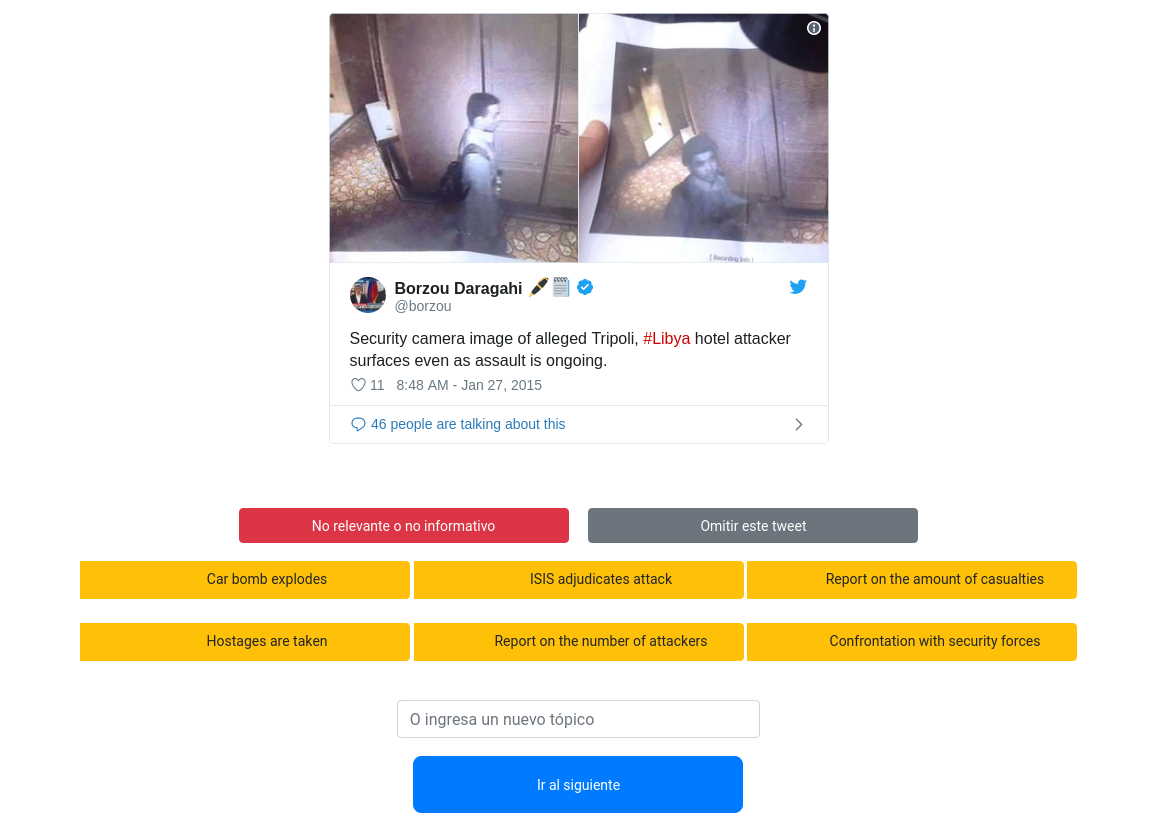
\includegraphics[width=.8\textwidth]{figures/url-model/label.png}
    \caption[Web interface for labeling tweets.]
    {Web interface for labeling tweets. In the top section a tweet is displayed.
    In the middle section, a list of options is displayed: a topic for each
    button, plus the option to mark a tweet as {\it non relevant or not
    informative}, or to skip it. In the bottom part of the interface, there is
    the possibility to add a custom topic, and then to continue with the next
    tweet. The user can select as many topics as they desire.}\label{fig:gt-web} \end{figure}%

\paragraph{Ground-truth generation.}
%
Sixteen people --mainly Computer Science undergrad and grad students-- labeled
tweets independently using a custom Web interface.
%
The interface displayed a tweet and a list of labels, and each user could assign
one or more labels to a tweet, mark the tweet as ``non relevant or not
informative'', or skip it if unsure (Figure~\ref{fig:gt-web}).
%
Some tweets may refer to more than one sub-topic, so we preferred that users
felt free to assign as many labels as they prefer.
%
The action of a user assigning labels to a tweet is referred as an evaluation,
and we imposed a limit of three evaluations per tweet.
%
This way, if three users evaluate the same tweet, that tweet will not be showed
again in the interface.

% \begin{center}
% \noindent\fbox{% 
%   \parbox{.95\textwidth}{% 
%   \it
%   The goal of this task is to assign descriptive labels to tweets.
%   %
%   With these labels we can validate a methodology to model news information
%   using tweets.

%   There are three news events available, described below. 
%   %
%   The corresponding tweets can be relevant to the event (by describing some
%   aspect of it), or not (e.g, spam, conversations).

%   %%

%   For example, if the event is an earthquake, a relevant tweet is one that 
%   informs about the magnitude, the casualties, etc.
%   %
%   A irrelevant or non informative tweet could mention the word ``earthquake'',
%   but do not describe anything about the event, or it is about something else
%   and not about the target event.
  
%   %%

  
%   Te pedimos seguir los pasos descritos abajo, y luego, al comenzar la tarea:
  
%   Escoger el o los tópicos más apropiados para cada tweet (puedes elegir más de
%   uno) Si no encuentras el tópico que crees que corresponde, puedes escribirlo
%   en el campo de texto correspondiente Si consideras que el tweet no entrega
%   información sobre el evento, o bien es totalmente irrelevante a éste, presiona
%   "No relevante o no informativo" Si no estás seguro/a de qué hacer, presiona
%   "Omitir este tweet" Si estás listo/a para continuar, presiona "Enviar" Repite
%   el proceso para el siguiente tweet Tras unos 20 o 30 minutos, vuelve a esta
%   página y pasa al siguiente evento. Estas instrucciones también están
%   disponibles en la interfaz de la tarea. Si tienes problemas con algunas
%   palabras en inglés, puedes usar algún recurso externo (como Google Translate)
%   para ayudarte. También puedes hacer click en los enlaces presentes en cada
%   tweet, pero consideramos que no es necesario. Precaución ya que algunos
%   enlaces pueden ya no estar disponibles o apuntar a sitios potencialmente
%   maliciosos.
  
%   Te pedimos al menos una hora para etiquetar tweets (unos 20 a 30 minutos por
%   cada evento).
  
%   No es necesario que destines una hora de corrido. Puedes salir y volver en
%   otro momento usando el mismo usuario y clave.
  
%   Entre más tweets etiquetes, ¡mucho mejor para nuestra evaluación! Muchas
%   Gracias :-)

%   }%
% }
% \end{center}



%
We manually generated the list of labels to be displayed in the interface by
looking into news reports in the Web.
%
The lists of labels are the following:

\begin{itemize}
  \item {\bf Libya Attack:}
  \begin{enumerate}
    \item {\it Car bomb explodes}
    \item {\it ISIS adjudicates attack}
    \item {\it Report on the amount of casualties}
    \item {\it Hostages are taken}
    \item {\it Report on the number of attackers}
    \item {\it Confrontation with security forces}
  \end{enumerate}
  \item {\bf Nepal Earthquake:}
  \begin{enumerate}
    \item {\it Avalanche in Mount Everest}
    \item {\it Death toll}
    \item {\it Reports on the magnitude of the earthquake}
    \item {\it Rescue of people}
    \item {\it Ways to help}
    \item {\it International aid}
    \item {\it Destruction of historical buildings}
    \item {\it Humanitarian crisis}
    \item {\it Destruction of buildings}
    \item {\it Replicas of the earthquake}
  \end{enumerate}
  \item {\bf Pistorius Trial:}
  \begin{enumerate}
    \item {\it Oscar Pistorius apologizes}
    \item {\it Oscar Pistorius vomits on court}
    \item {\it Oscar Pistorius removes his prosthesis}
    \item {\it Psychiatric evaluation}
    \item {\it Final arguments}
    \item {\it Pistorius pledges innocence}
    \item {\it Paddy Powers}
    \item {\it Witnesses}
    \item {\it Police under investigation}
    \item {\it Interrogatory}
    \item {\it Shooting in a restaurant}
  \end{enumerate}
\end{itemize}

To select the tweets to be displayed in the interface, we first removed all
duplicated tweets.
%
For this, we only considered the text in the tweets, but not the URLs.
%
This way, all the tweets sharing the same text would receive the same labels.
% 
Then, we distributed the resulting tweets in the interface in such a way that
there were roughly no underrepresented sub-topics.
%
For this, we manually produced a list of keywords for each label, and for each
label ranked the tweets using Okapi BM25;  in the interface, a random label was
chosen and the corresponding ranked tweet was presented.


Finally, to assign a ground-truth label to a tweet, we selected the label users
chose the most for that tweet.
%
This resulted in 401 labeled tweets (1339 labels in total) for the Libya event,
368 (531 labels) for Nepal, and 85 (362 labels) for Pistorius.

%%

\paragraph{Validation using clustering.}
%
As our goal is to compare event representations, we chose k-means as a simple
baseline to validate the effectiveness of our model.
%
To find sub-topics, we ran k-means with different numbers of clusters, using our
representation and raw tweets.
%
For the baseline, we considered each tweet as a document, that is, we computed
the sum of word vectors for each tweet individually.
%
We report normalized mutual information, purity, and entropy for each event,
using the available labels in both settings (Figures~\ref{fig:purity},
\ref{fig:nmi}, \ref{fig:entropy}).
%
Note that the measures were done only on the labeled tweets, that is, as if the
unlabeled tweets did not exist in the clustering solution.

%%

We observe that with our representation, the clustering outperforms the baseline
in most cases. 
%
In the case of the Nepal event, our representation had better purity, NMI and
entropy. 
%
In the case of Pistorius, the measures are very similar. 
%
However, in the case of Libya, our representation matches the baseline after a
certain number of clusters, except in the entropy measure
(Figure~\ref{fig:entropy}).
%
We believe this is because the Libya event has more unrelated (spam and
irrelevant) tweets, and the model captures more information about unrelated
topics, as they use more URLs.
%
And in terms of running time, we observed that k-means under the representation
runs one order of magnitude faster than the baseline (Figure~\ref{fig:times}). 
%
These results suggest that our representation is capable of preserving topical
information about the target event, with reduced time required to identify this
kind of information. 
%

\begin{figure}
  \centering
  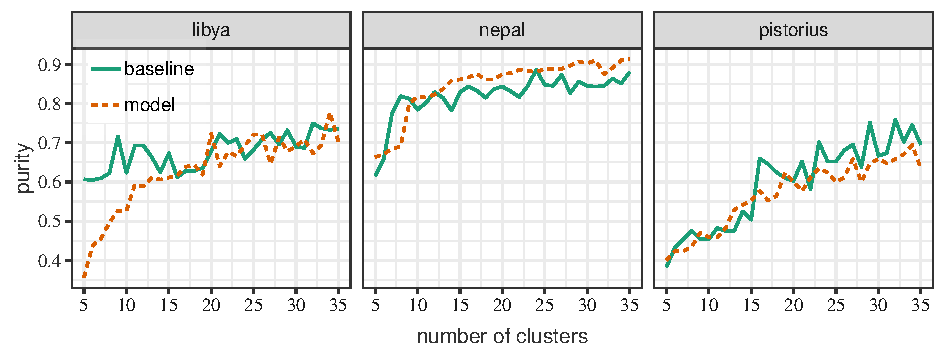
\includegraphics[width=\textwidth]{figures/url-model/purity}
  \caption{Purity for different numbers of clusters computed from each event.}\label{fig:purity}
\end{figure}%

\begin{figure}
    \centering
    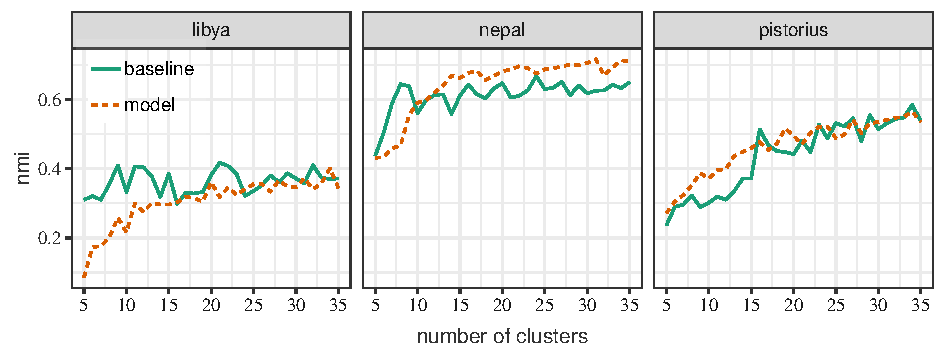
\includegraphics[width=\textwidth]{figures/url-model/nmi} 
    \caption{Normalized Mutual Information for different numbers of clusters computed from each event.}\label{fig:nmi}
\end{figure}

\begin{figure}
  \centering
  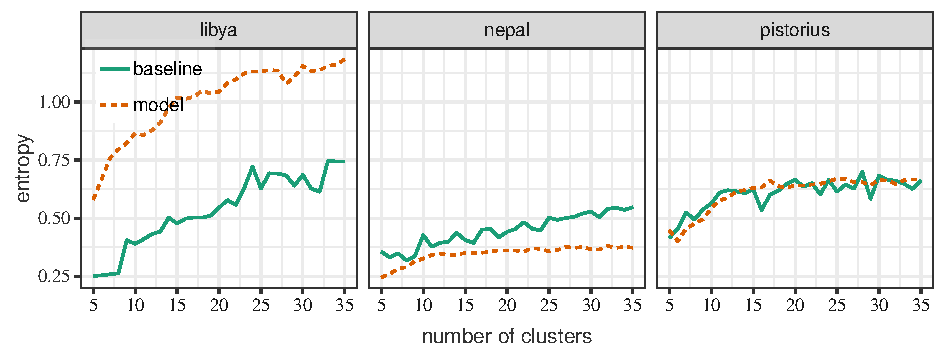
\includegraphics[width=\textwidth]{figures/url-model/entropy} 
  \caption{Entropy for different numbers of clusters computed from each event.}\label{fig:entropy}
\end{figure}


\begin{figure}
  \centering
  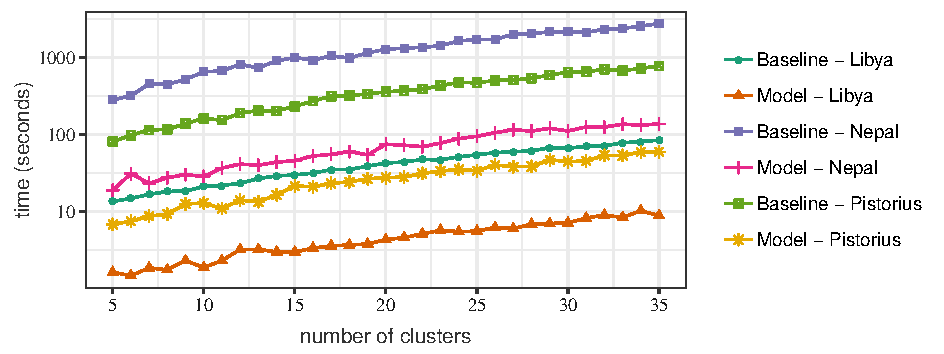
\includegraphics[width=\textwidth]{figures/url-model/times}
  \caption{Running times for clustering for each event.}\label{fig:times}
\end{figure}%

\section{Discussion}\label{sec:conclusions}

% %

% %

%%
% In a future work, we are interested in studying new strategies to represent
% external URLs using social media data, and how this can be used to better
% understand real-world events.


In this chapter, we presented a lightweight representation to represent newsworthy
information in social media, and a methodology to generate a representation from
a set of social media messages. 
%
Our representation leverages the use of shared URLs in the context of news
events to aggregate common information across messages, and allows us to
identify sub-topics in an event much faster than traditional or off-the-self
methods.
%
We observed that our representation is capable to preserve topical information
of an event.
%
At the same time, it is suitable to be significantly smaller than the original
dataset, requiring much less computational resources to perform standard tasks.
%
This representation requires little data preprocessing, meaning that is
convenient to use in an scenario of having large, raw, uncurated data.
%
However, there is room for improvement in terms of the results.
%
For this, we need to perform a large scale evaluation, although it is hard to
find ground truth data for large, raw, un-curated social media
messages~\cite{Alonso:2015:WCW:2740908.2745397}.
%
For this case scenario, our methodology aims to help processing large quantities
of noisy, un-curated data around news events more effectively.
%
In future work we are interested in studying how to formally define and identify
topic-specific URLs in the events, which we believe are key to creating a useful
representation.
%
%We are also interested in looking for different strategies to represent
%topics in news events by aggregating content using external URLs on social media.
%
